
%...........................................................................................
\paragraph{Experiment 1}

This benchmark originates in \cite{dohu03}. It is also carried out in \cite{bepo10}.
It considers the advection of a product-cosine hill
in a prescribed velocity field. The initial temperature is:
\begin{equation}
T_0(x,y)=
\left\{
\begin{array}{cc}
\frac{1}{4}
\left(1+\cos \pi\frac{x-x_c}{\sigma}\right)
\left(1+\cos \pi\frac{y-y_c}{\sigma}\right)
& \text{if } (x-x_c)^2+(y-y_c)^2\leq \sigma^2 \\
0 & \text{otherwise}
\end{array}
\right.
\end{equation}
The boundary conditions are $T(x,y)=0$ on all four sides of the unit square domain. In what follows we set $x_c=y_c=1/6$ and $\sigma=0.2$.  The velocity field is analytically prescribed: $\vec\upnu=(-(y-y_c),+(x-x_c))$.

In what follows we test the time integration scheme by setting $\alpha_T=1$ (fully implicit formulation), $\alpha=0$ (fully explicit formulation) and $\alpha_T=1/2$ (Crank-Nicolson).  
In the book Donea \& Huerta set the timestep is set to $\delta t=2\pi/200$ which corresponds to a CFL number of approximately 0.666. If we want to be able to run this experiment at higher 
resolution we need to adapt the timestep to the mesh size (CFL criterion). We therefore set the CFL number to 0.5 and compute $\delta t$ accordingly (see Section~\ref{ss:cfl}).  
The density and heat capacity values are set to 1. We monitor the minimum and maximum value of the temperature field, as well as the total thermal energy $E_T$ in the 
system during the full rotation:
\[
E_T=\int_\Omega \rho_0 C_p T dV = \int_\Omega T dV = |\Omega| \langle T \rangle 
\qquad
\text{where}
\qquad
\langle T \rangle = \frac{1}{|\Omega|} \int_\Omega T dV
\]
The time evolution of the temperature with the Crank-Nicolson algorithm is shown hereunder:
\begin{center}
a)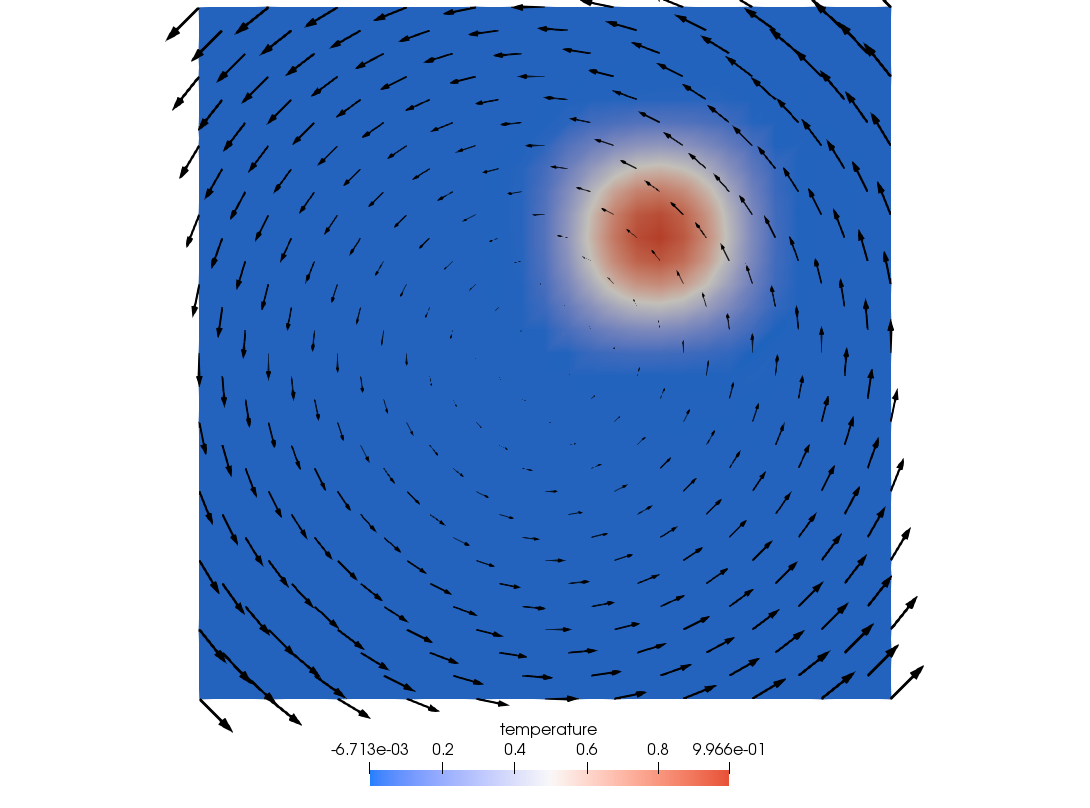
\includegraphics[width=4.8cm]{python_codes/fieldstone_43/results/crni/velfield}
b)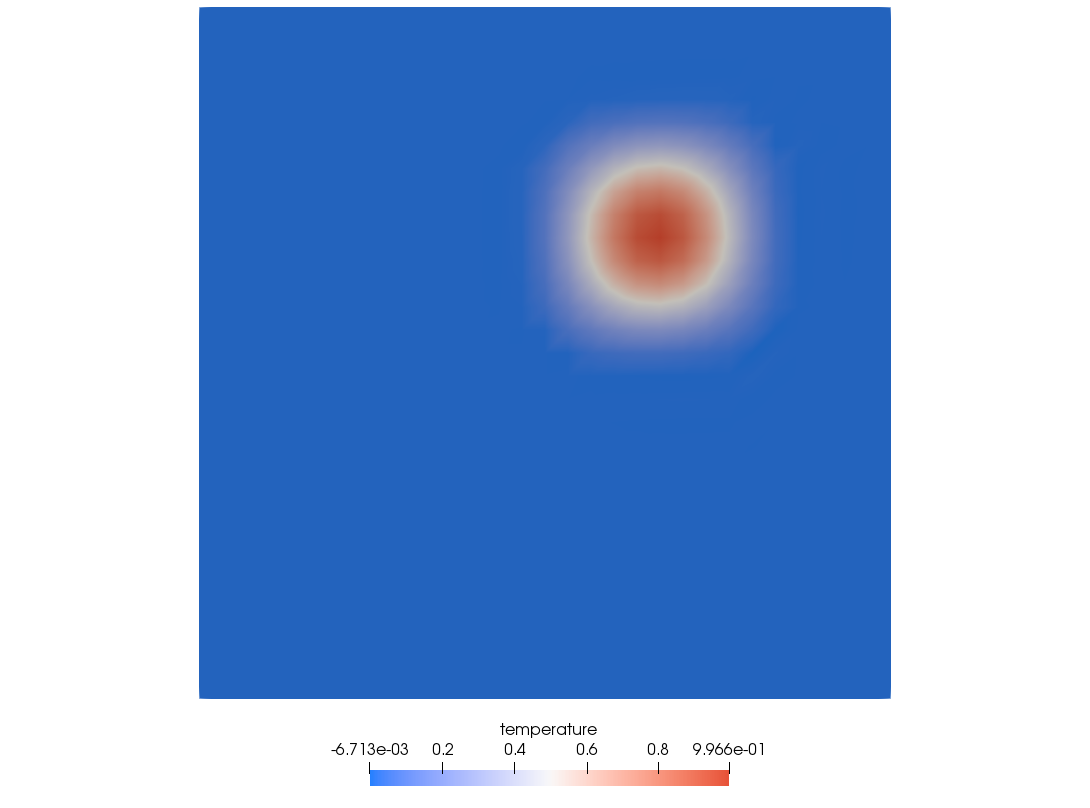
\includegraphics[width=4.8cm]{python_codes/fieldstone_43/results/crni/crnitemp0000}
c)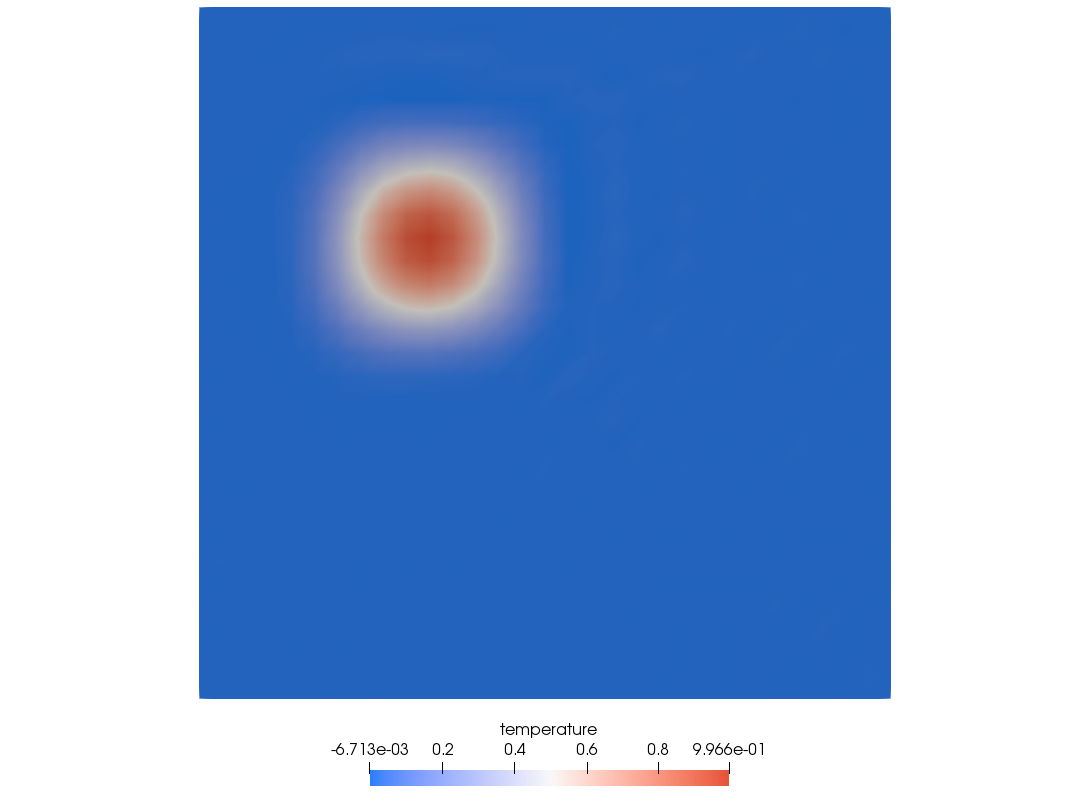
\includegraphics[width=4.8cm]{python_codes/fieldstone_43/results/crni/crnitemp0050}\\
d)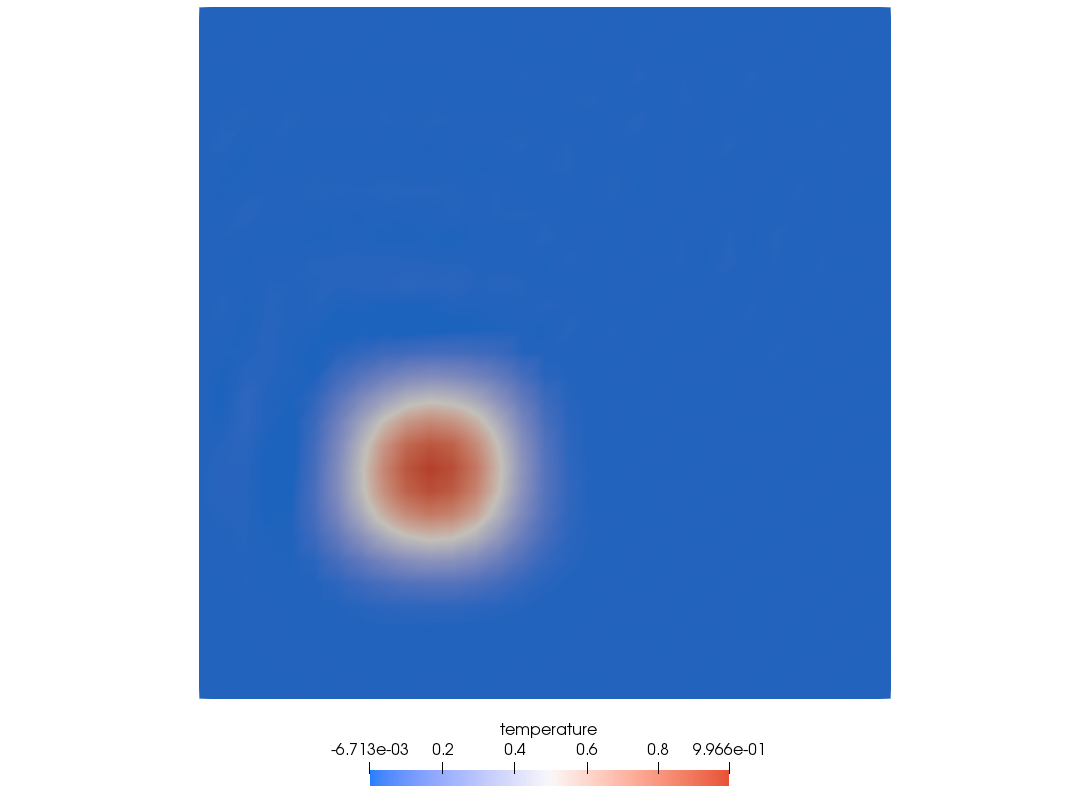
\includegraphics[width=4.8cm]{python_codes/fieldstone_43/results/crni/crnitemp0100}
e)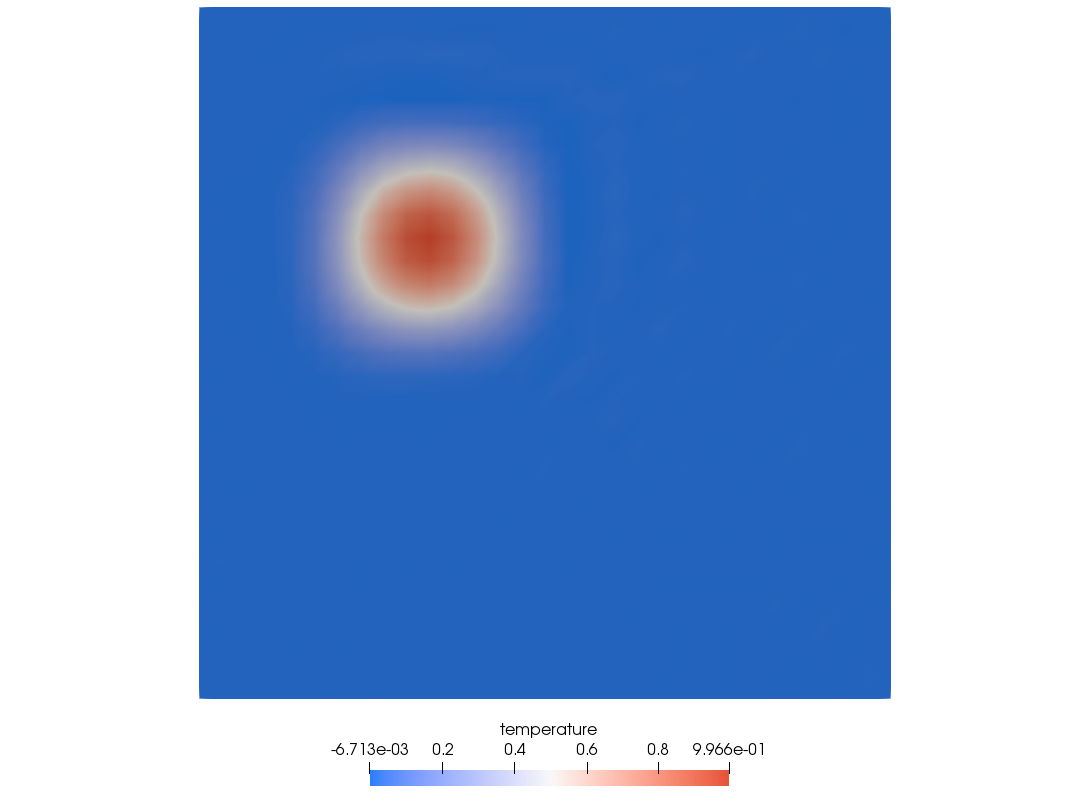
\includegraphics[width=4.8cm]{python_codes/fieldstone_43/results/crni/crnitemp0050}
f)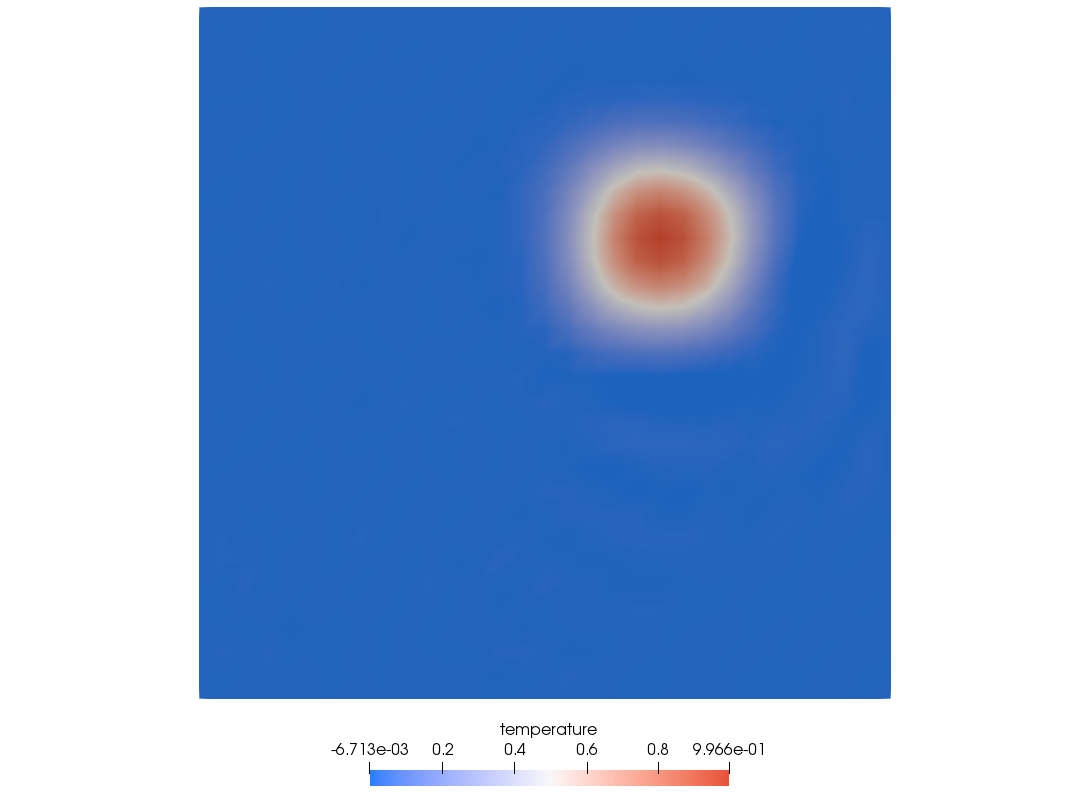
\includegraphics[width=4.8cm]{python_codes/fieldstone_43/results/crni/crnitemp0199}\\
{\small a) Velocity field and initial temperature; b,c,d,e,f) Temperature field throughout the rotation.} 
\end{center}
Turning now to the statistics, we plot $\min(T)$, $\max(T)$ and $E_T$ as a function of time:
\begin{center}
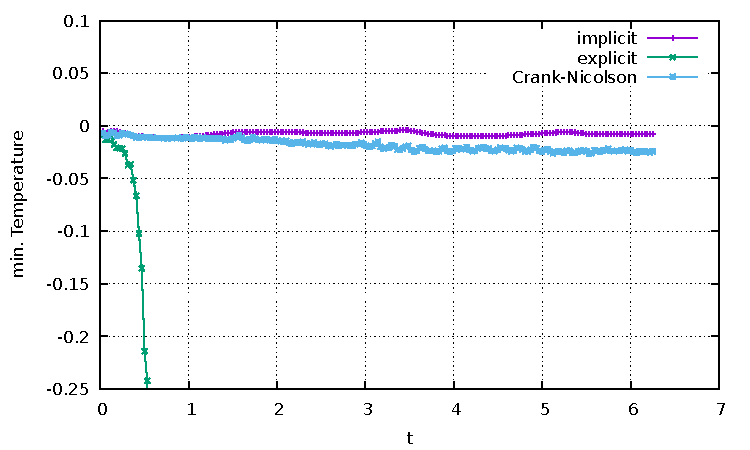
\includegraphics[width=5cm]{python_codes/fieldstone_43/results/Tmin.pdf}
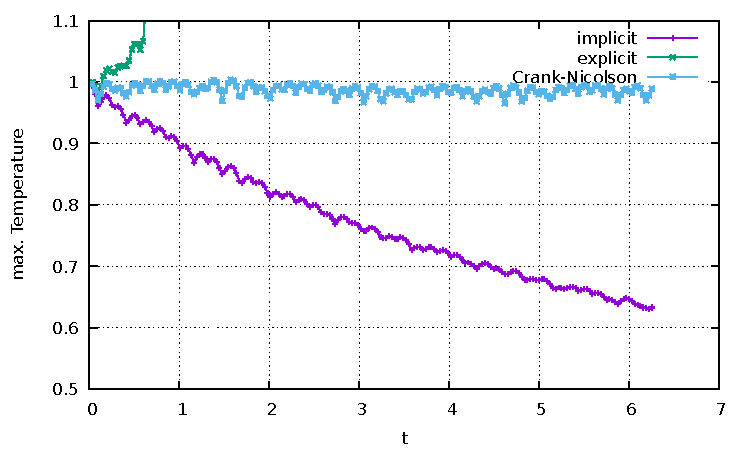
\includegraphics[width=5cm]{python_codes/fieldstone_43/results/Tmax.pdf}
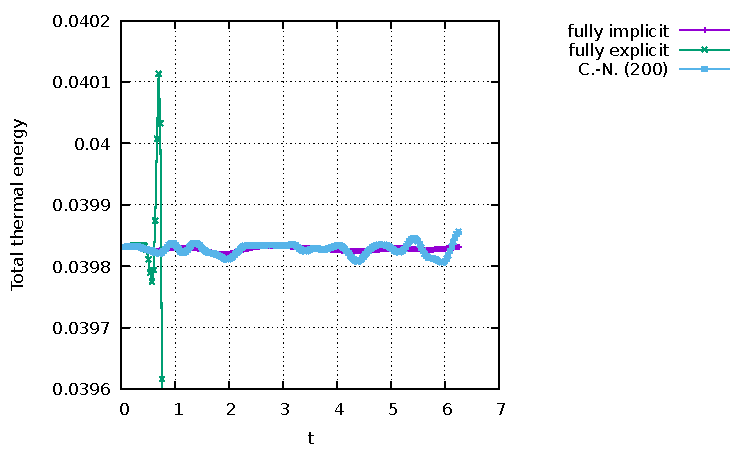
\includegraphics[width=5cm]{python_codes/fieldstone_43/results/ET.pdf}\\
{\small Time evolution of the min and max temperature and the total energy}
\end{center}
The conclusions are clear: the explicit method diverges quickly and is unusable. The fully implicit and Crank-Nicolson 
method yield similar energy conservation but the fully-implicit showcases a clear loss in maximum temperature as shown in the following figure:
\begin{center}
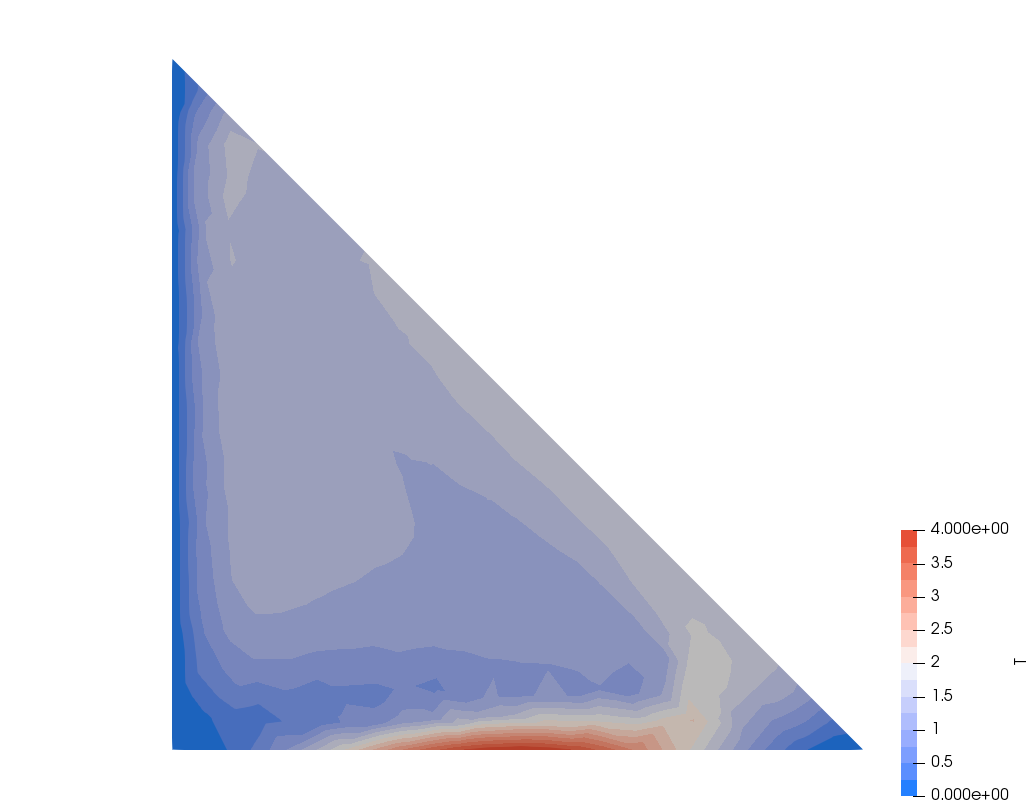
\includegraphics[width=15cm]{python_codes/fieldstone_43/results/temp}\\
{\small Temperature field after a full rotation with isocontours every 0.1 value.\\ Left: Fully-implicit; Right: Crank-Nicolson}
\end{center}

Finally we can run the experiment (still a $2\pi$ rotation) 
with three different time steps ($\delta t=2\pi/30,2\pi/60,2\pi/120$) 
and we recover very similar results to those presented in \cite{dohu03}:

\begin{center}
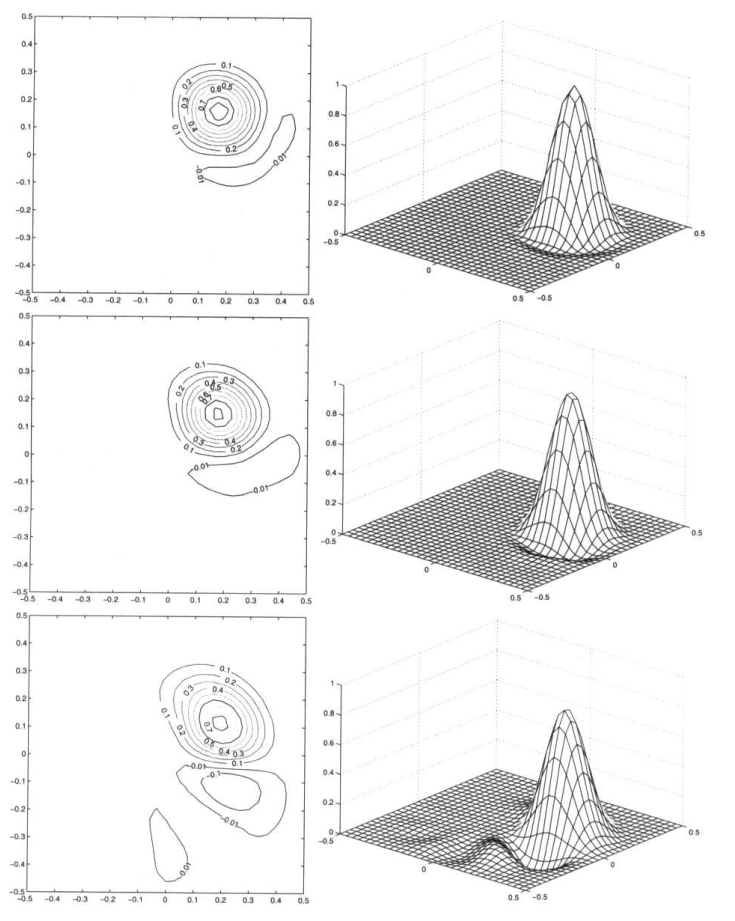
\includegraphics[height=8cm]{python_codes/fieldstone_43/results/dohu03}
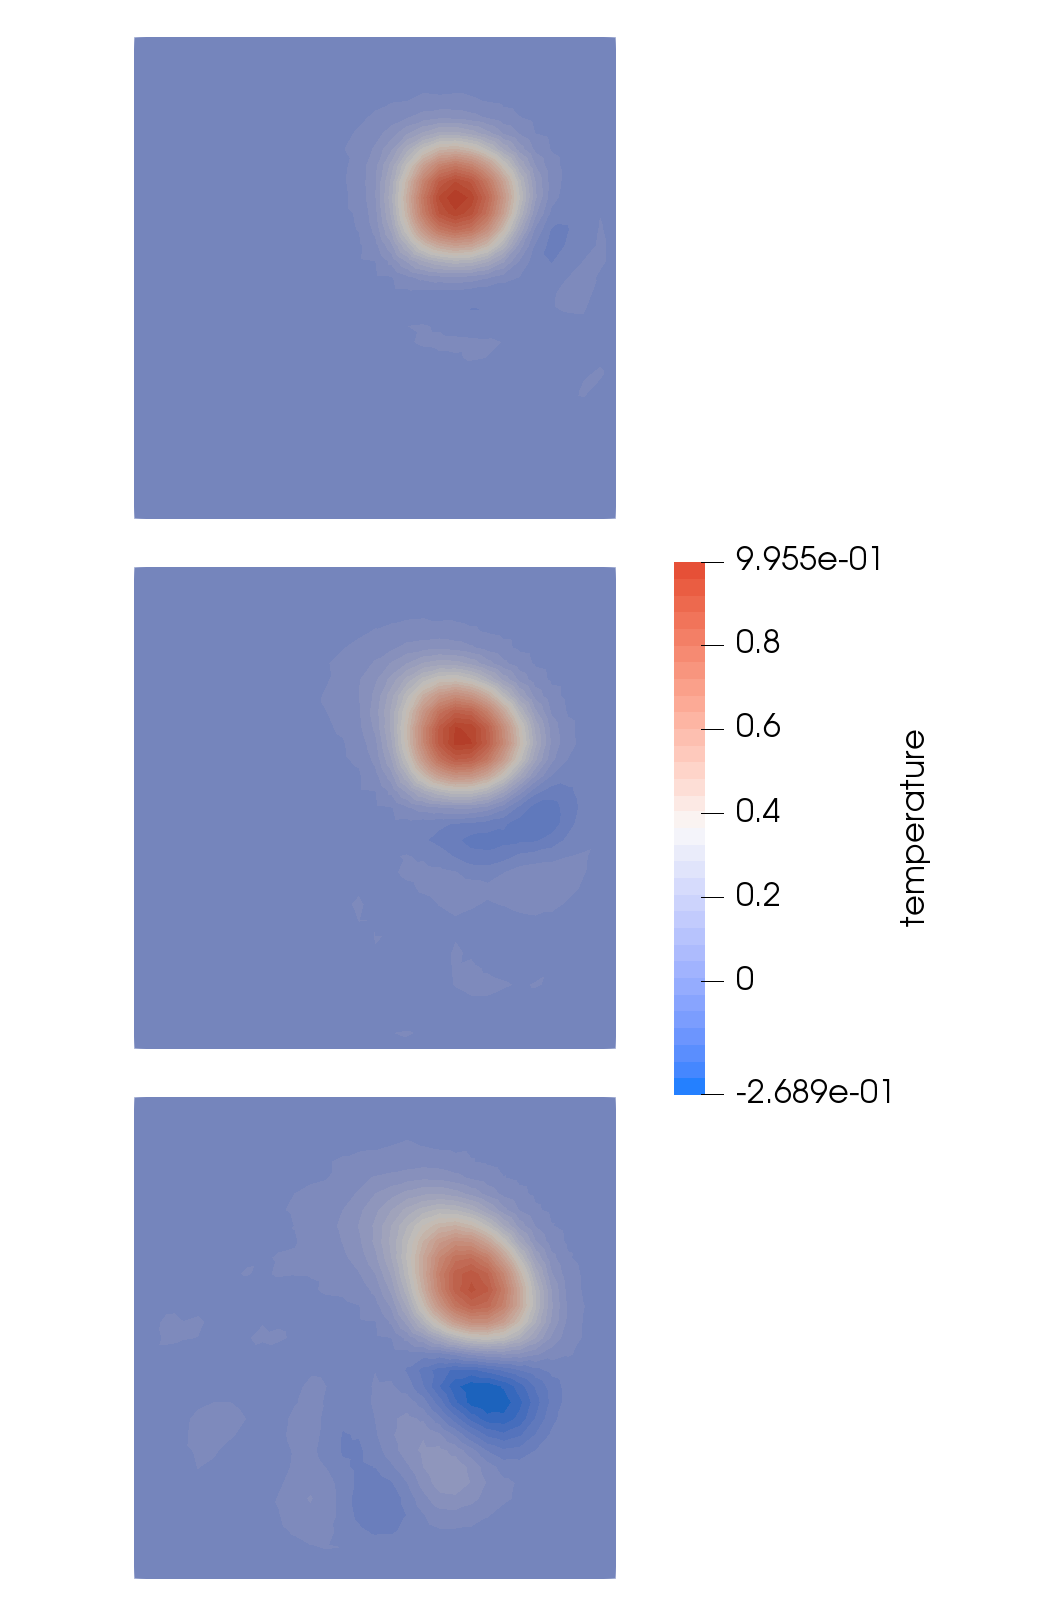
\includegraphics[height=8cm]{python_codes/fieldstone_43/results/temps_30_60_120}\\
{\small From top to bottom: $\delta t=2\pi/120,2\pi/60,2\pi/30$ with Crank-Nicolson. Left panel is taken from donea \& Huerta \cite{dohu03}}
\end{center}

\begin{center}
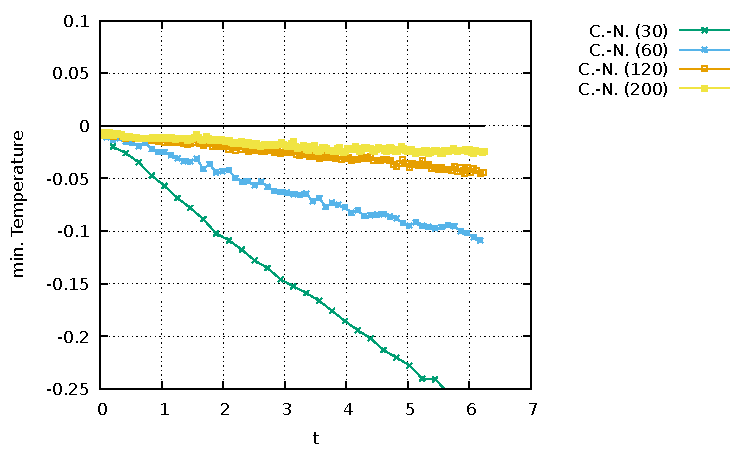
\includegraphics[width=5cm]{python_codes/fieldstone_43/results/Tmin_CN.pdf}
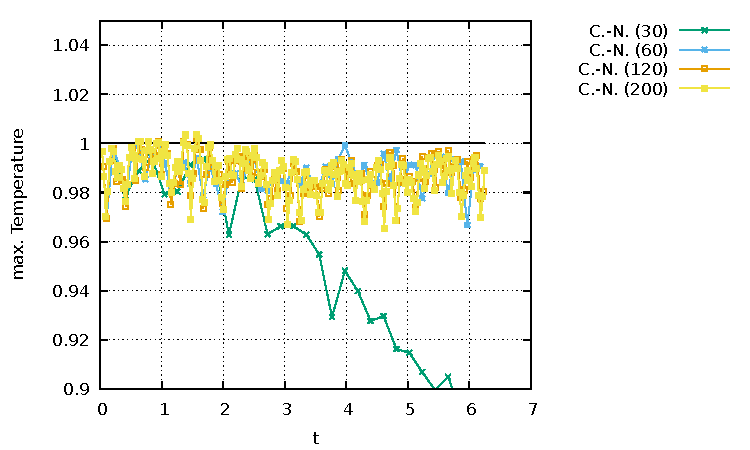
\includegraphics[width=5cm]{python_codes/fieldstone_43/results/Tmax_CN.pdf}
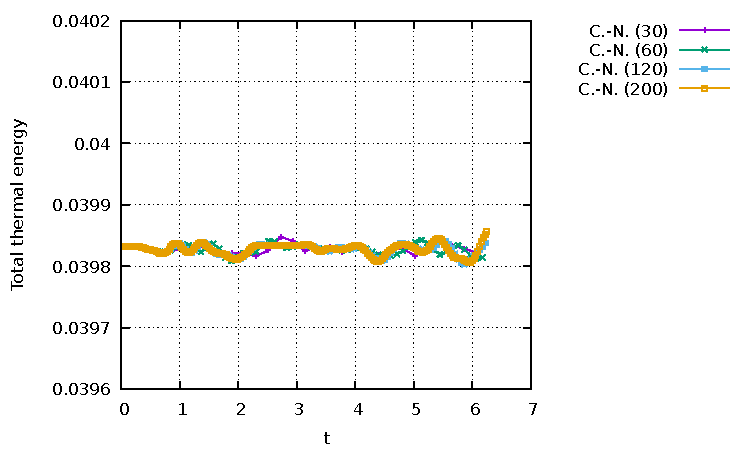
\includegraphics[width=5cm]{python_codes/fieldstone_43/results/ET_CN.pdf}\\
{\small Time evolution of the min and max temperature and the total energy obtained with the Crank-Nicolson algorithm for 4 values of the timestep as indicated by the number between parenthesis.}
\end{center}


\begin{center}
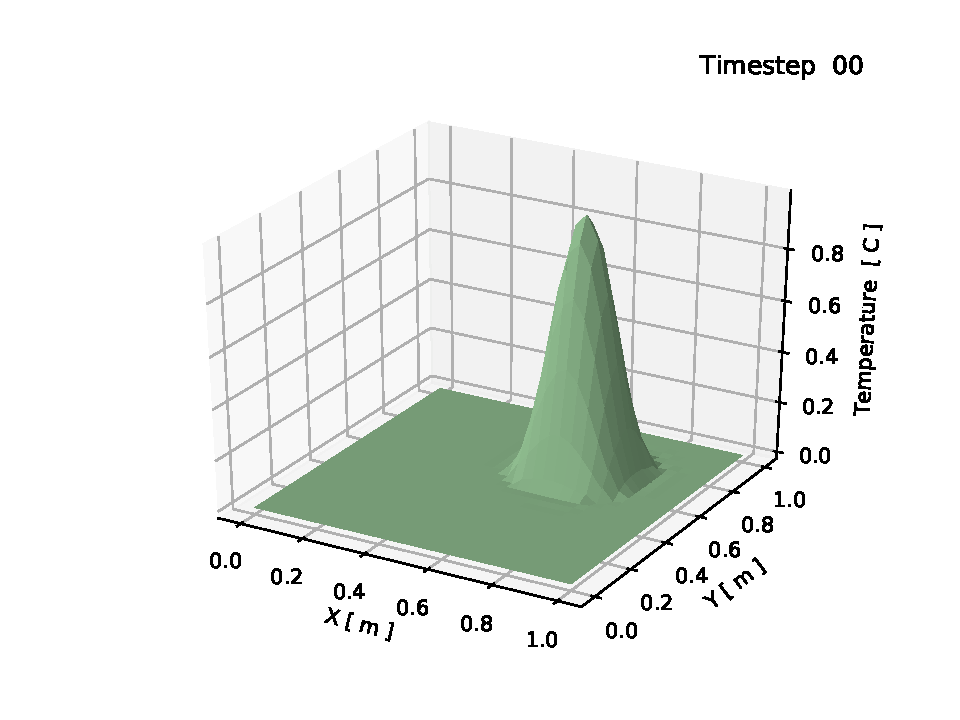
\includegraphics[width=3cm]{python_codes/fieldstone_43/results/solution_0000.pdf}
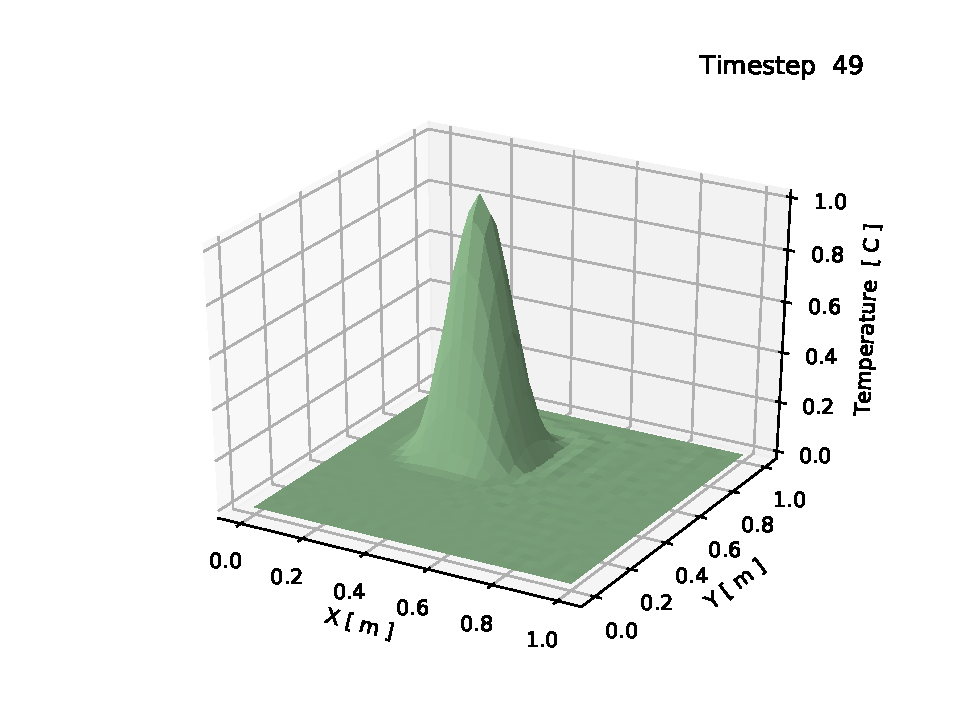
\includegraphics[width=3cm]{python_codes/fieldstone_43/results/solution_0049.pdf}
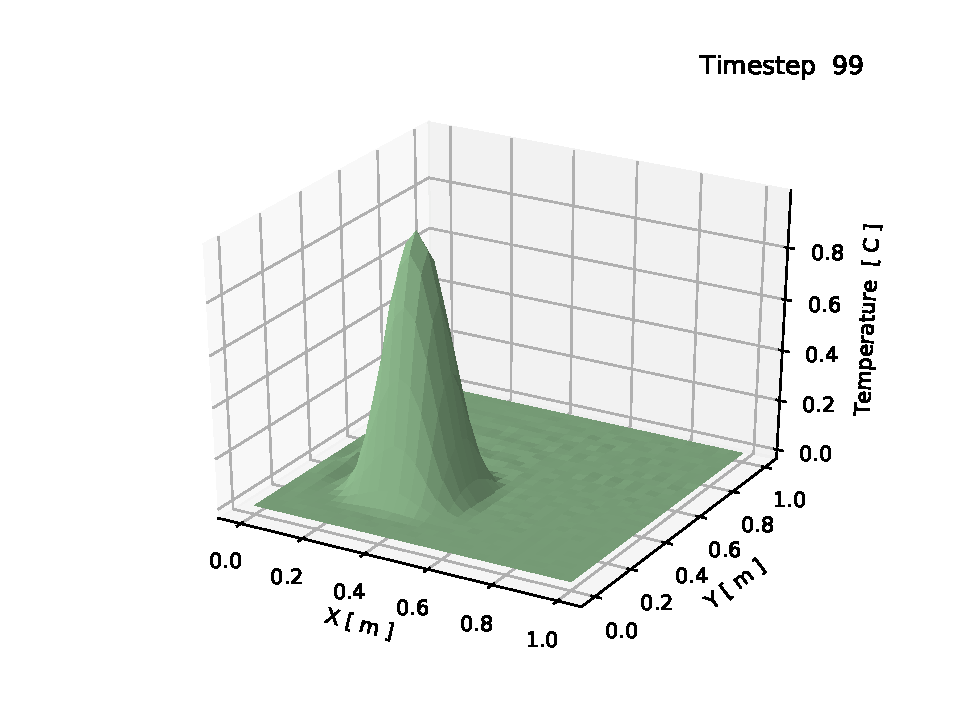
\includegraphics[width=3cm]{python_codes/fieldstone_43/results/solution_0099.pdf}
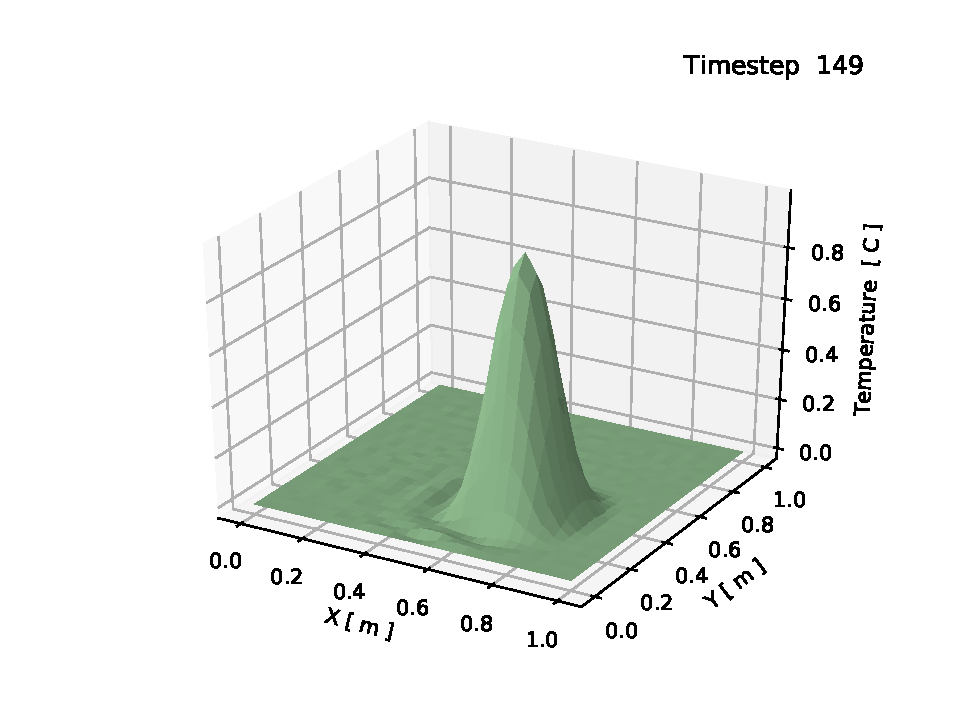
\includegraphics[width=3cm]{python_codes/fieldstone_43/results/solution_0149.pdf}
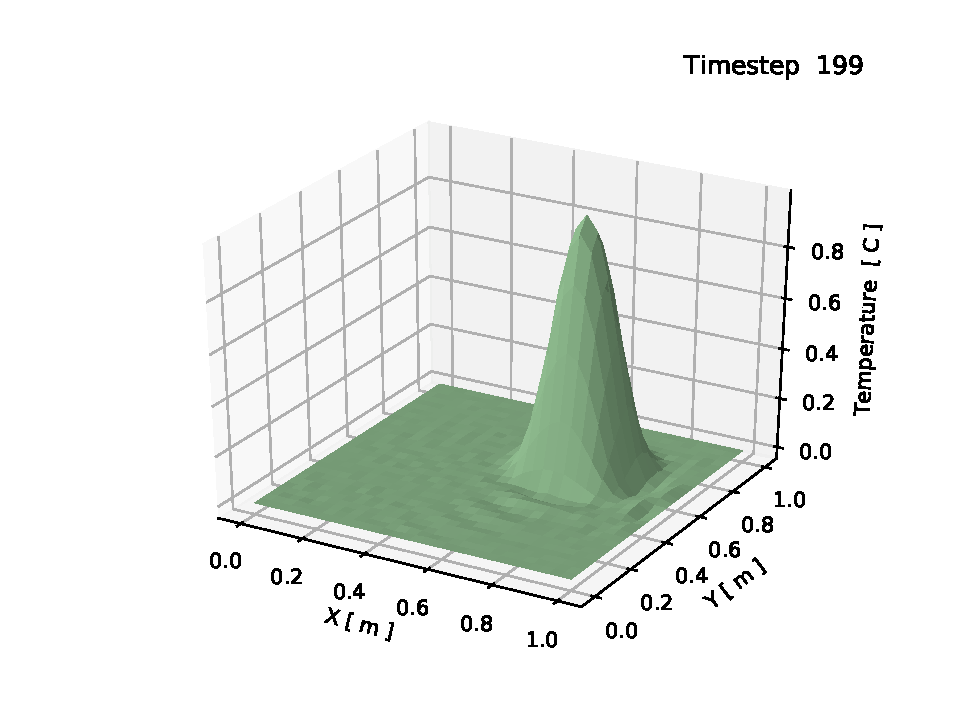
\includegraphics[width=3cm]{python_codes/fieldstone_43/results/solution_0199.pdf}\\
{\small Time evolution of the temperature field for $\delta t=2\pi/200$ with Crank-Nicolson.}
\end{center}

I have also implemented BDF1,2,3,4,5. BDF2 outperforms BDF1 and is comparable to C-N. 
For reasons unknown to me, the BDF3 diverges after 100 time steps. So do 
BDF4 and BDF5 after even less timesteps. In the following picture the temperature is shown for 
BDF1,2,3 and Crank-Nicolson after a full rotation.

\begin{center}
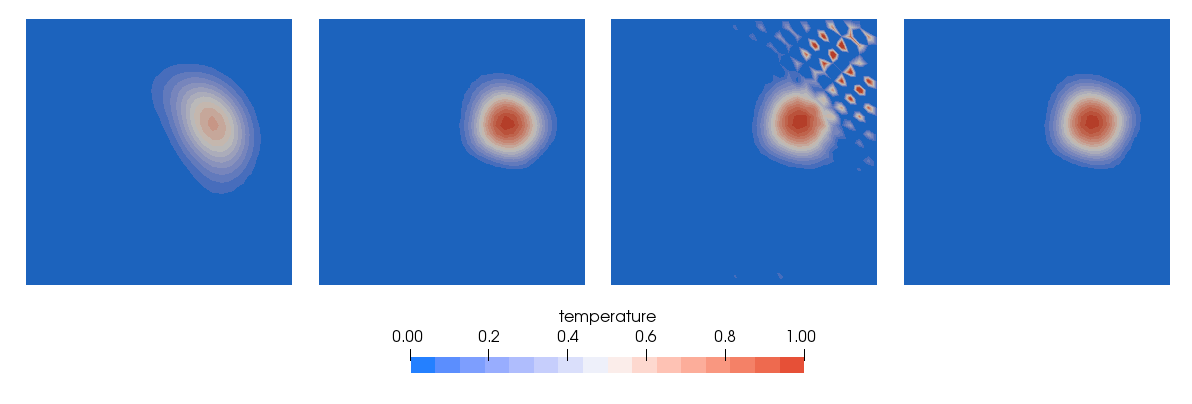
\includegraphics[width=15cm]{python_codes/fieldstone_43/results/Tbdf123crni.png}\\
{\captionfont Left to right: BDF1 (i.e. implicit euler), BDF2, BDF3, Crank-Nicolson}
\end{center}

I now turn to another aspect of this problem: what is the effect of the SUPG stabilisation 
scheme on the solution? In what follows Crank-Nicolson is used, only the resolution is increased. 
We see that using SUPG introduces a lot of diffusion and it smears out the cone, to the 
point that the maximum Temperature value after a full rotation is below 1/2. Increasing resolution 
helps mitigating the effect.
On the other hand the minimum value stays closer to zero when SUPG is used. 

\begin{center}
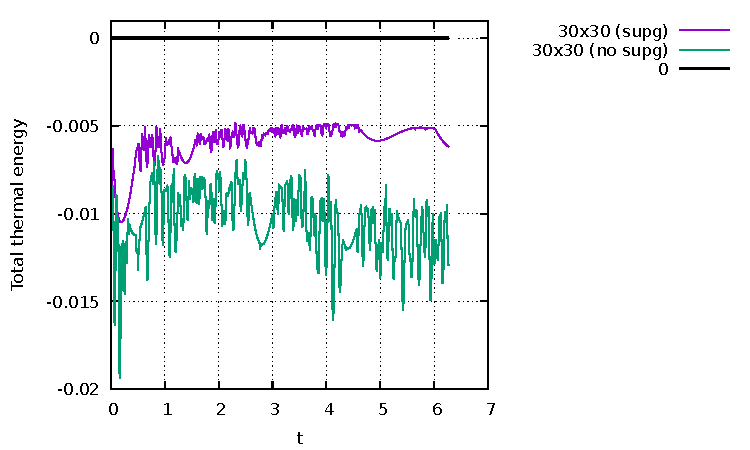
\includegraphics[width=6cm]{python_codes/fieldstone_43/results/Tmin_supg}
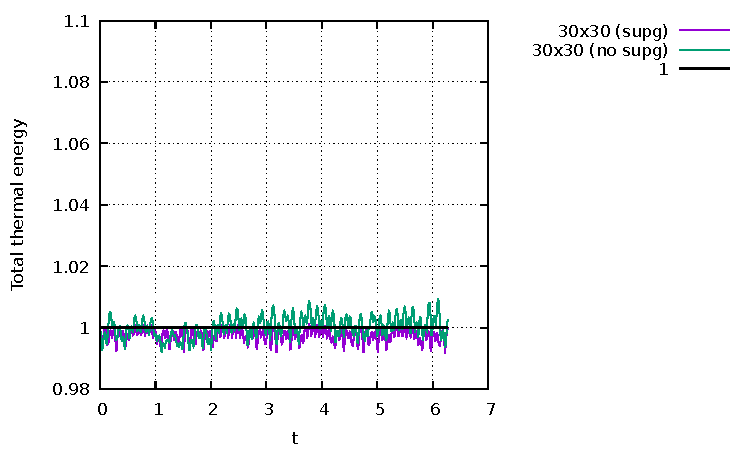
\includegraphics[width=6cm]{python_codes/fieldstone_43/results/Tmax_supg}\\
\includegraphics[width=15cm]{python_codes/fieldstone_43/results/T_supg}\\
{\captionfont From left to right: 30x30, 40x40, 50x50, 60x60, 80x80. Note the scale from 0 to 0.5}
\end{center}

%...........................................................................................
\paragraph{Experiment 2}

This setup is inspired by the one in the ASPECT manual. The cone is now replaced by three 
'objects' : a Zalesak disk \ref{}, a sharp cone and a truncated cosine hill:

\begin{lstlisting}
   for i in range(0,nnp):
       T[i]=0.
       xi=x[i]
       yi=y[i]
       if np.sqrt((xi-0.5)**2+(yi-0.75)**2)<0.15 and (np.abs(xi-0.5)>=0.025 or yi>=0.85):
          T[i]=1
       if np.sqrt((x[i]-0.5)**2+(y[i]-0.25)**2)<0.15:
          T[i]=1-np.sqrt((x[i]-0.5)**2+(y[i]-0.25)**2)/0.15
       if np.sqrt((x[i]-0.25)**2+(y[i]-0.5)**2)<0.15:
          T[i]=0.25*(1+np.cos(np.pi*np.sqrt((xi-0.25)**2+(yi-0.5)**2)/0.15))
\end{lstlisting}

\begin{center}
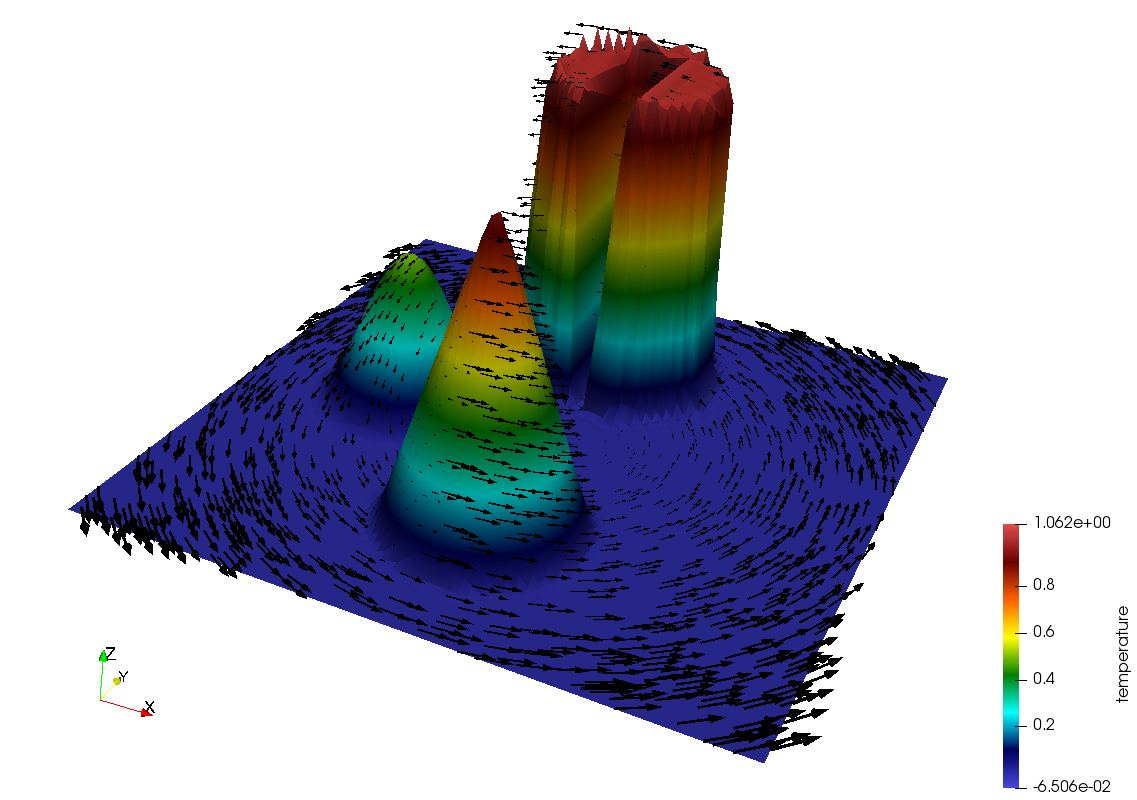
\includegraphics[width=8cm]{python_codes/fieldstone_43/buildings}
\end{center}

For this experiment the CFL number is set to 0.1

%...........................................................................................
\paragraph{Experiment 3}




